\chapter{Contributions to the Practical Course Microservice2Go}
\label{cha:m2go}

M2Go (Microservice2Go) is a practical course, which supplements the lecture
WASA1 (Web Applications and Service-oriented Architectures 1). WASA1 is offered
by the research group C\&M (Cooperation \& Management) each winter semester.
The lecture WASA1 covers the development and architecture of advanced web
applications that employ microservices and the cloud. M2Go supplements the
lecture by applying the learned concepts from the lecture to a concrete example
for which microservices are implemented using the Golang programming language.
The course will be offered each winter semester starting with the winter
semester of 2023/2024. M2Go is further described in Section
\ref{sec:m2g_description}. Section \ref{sec:m2g_operation} describes the
operations of M2Go. During the duration of this thesis, the author contributed
to the preparation of this course. These contributions are described in Section
\ref{sec:m2g_contribution}. Part of the author's contributions was the
preparation of exercises for the participants of M2Go. 
Section \ref{sec:m2g_description_exercises} contains a description of the different exercises that were created
and their purpose. The prepared chapter with the exercises which will be used in the M2Go course material is placed in
Section \ref{sec:m2g_exercise}. Section \ref{sec:m2g_infrastructure} contains
a challenge that will be an optional exercise in M2Go.
Section \ref{sec:m2g_solutions} contains the solutions to the exercises.

\section{Description of the Practical Course Microservice2Go}
\label{sec:m2g_description}

\begin{figure}[tb]
	\centering
	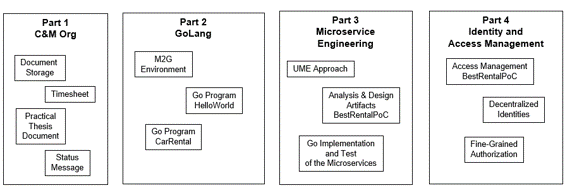
\includegraphics[width=\textwidth]{figures/m2go_parts.png}
	\caption{M2Go Parts \cite{CM-W-M2G}}
	\label{fig:m2go_parts}
\end{figure}

M2Go is split into four different parts which are illustrated in Figure
\ref{fig:m2go_parts}. The first part, C\&M Org, familiarizes the students with
the working processes of C\&M. Each student has a timesheet in which they track
the amount of time that they spend on the practical course. The students also
create a practical thesis document which is kept in the document storage of
C\&M. The practical thesis document is written throughout the practical course
and documents the tasks carried out by students and what they learned. It is
the main basis for their final grade. The work at C\&M is based on a bi-weekly
cycle that starts with the weekly status message. The status message is a
simple email from a student to the C\&M team to signal that they completed
their tasks for the week and that their practical thesis document as well as
the timesheet are in order. Every second week, each student has to provide a
version of their practical thesis document which is ready for review. This
review is discussed in the weekly project team meeting after which the student
updates their practical thesis document accordingly. In the Golang part, the
students are introduced to the Golang programming language. They start by
setting up their M2Go Environment for developing applications with Golang. This
is then used to create the first program called HelloWorld to get familiar with
the programming language. The goal of this program is to output the text
``Hello World!'' to the console which is a standard first program to develop
when learning any new language. Afterward, the program CarRental will be
developed which validates if a date is valid. This program teaches the students
the fundamentals of Golang like control structures and unit testing. Based on
the program CarRental, CarRentalCLI is developed. This program provides a basic
command-line input (CLI) to interact with a microservice called CarRental from
a C\&M research project. CarRentalCLI does not interact with a real
microservice but instead provides a local version of the service which is
implemented by the students. The Microservice Engineering part teaches students
how to develop microservices. The development process being used is the Unified
Microservice Engineering (UME) approach from C\&M. The microservices that will
be developed for this part stem from the Proof of Concept (PoC) BestRentalPoC.
Based on the UME approach, the needed microservices are first analyzed and
designed. Following the design, the microservices are then implemented and
tested using Golang by employing the knowledge which was gained in the previous
part. Identity and Access Management is the final part of M2Go. It covers the
topic of access management for BestRentalPoC by using decentralized identities
and fine-grained authorization. While this part is currently planned, it is not
yet ready.

\section{Operation of the Practical Course Microservice2Go}
\label{sec:m2g_operation}

\begin{figure}[tb]
	\centering
	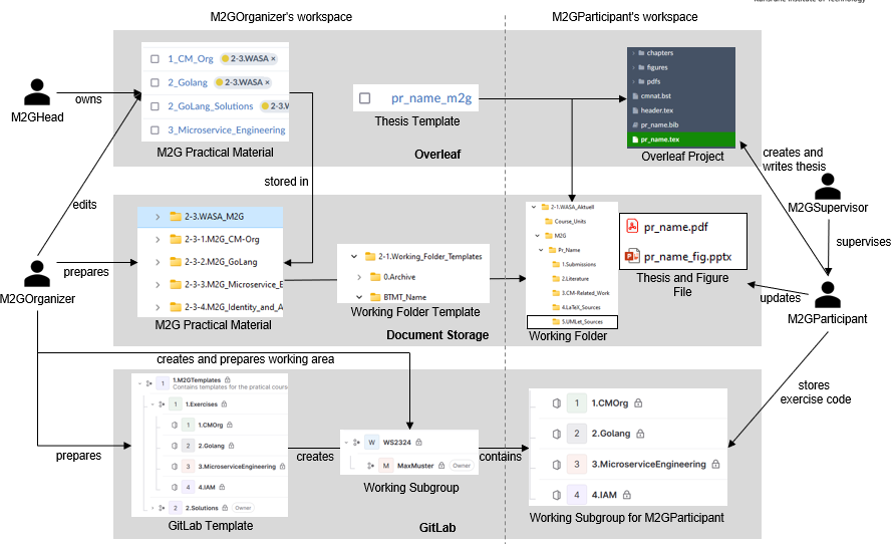
\includegraphics[width=\textwidth]{figures/m2go_actors_and_systems.png}
	\caption{M2Go Actors and Systems \cite{CM-W-M2G}}
	\label{fig:m2go_actors_and_systems}
\end{figure}

There are four actors in M2Go as seen in Figure
\ref{fig:m2go_actors_and_systems}. The M2GHead owns the M2Go course as well as
all of its materials and templates. The M2GHead is responsible for the course.
The M2G Practical Material is stored in the C\&M Document Storage. It is
prepared by the M2GOrganizer. The M2GOrganizer also creates the Working Folder
Template which is used to create the Working Folder for the M2GParticipants.
The working folder contains the sources and the current version of an
M2GParticipant's Practical Course Thesis. The Practical Course Thesis is
written in Overleaf and is based on the C\&M Thesis Template. The M2GOrganizer
also creates GitLab Templates for the different parts of the course. The
templates are used to create the GitLab repositories for the current semester's
course. M2GParticipants store their solutions to the exercises in the
corresponding GitLab repository. Finally, there is also the M2GSupervisor who
supervises and assists M2GParticipants. The M2GHead and M2GOrganizer are
responsible for grading each M2GParticipant's participation in the course. The
role of the author in the preparation of this course was that of an
M2GOrganizer who creates the master solutions to the exercises. Because the
course is currently being prepared and not yet offered, the author was not
responsible for any grades.

\begin{figure}[tb]
	\centering
	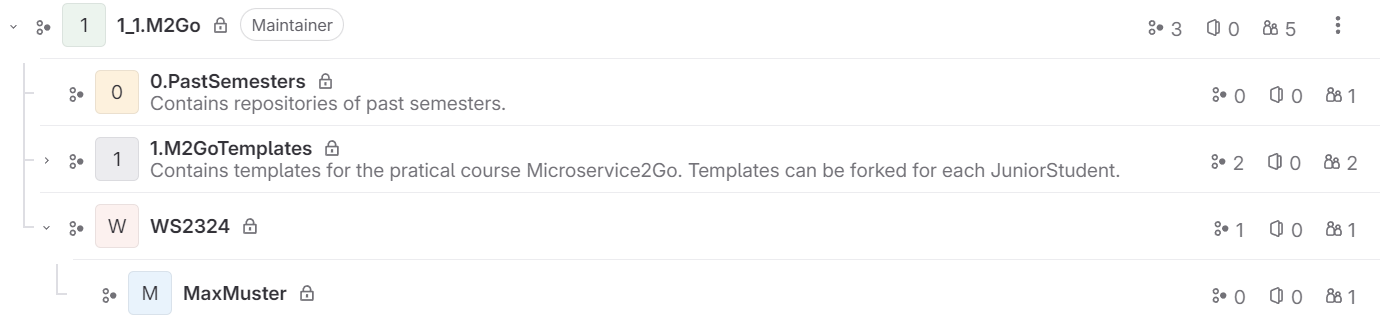
\includegraphics[width=\textwidth]{figures/m2go_gitlab.png}
	\caption{M2Go GitLab Repository Structure \cite{CM-G-M2G}}
	\label{fig:m2go_gitlab}
\end{figure}

The GitLab repository for M2Go is split into three sections. An overview of the
sections can be seen in Figure \ref{fig:m2go_gitlab}. 0.PastSemesters is meant
as an archive that contains the work from previous semesters. 1.M2GoTemplates
contains template repositories with the exercises for the course as well as
their solutions. WS2324 will contain a repository for each student who
participates in the course where they can store their solutions to the
exercises. M2GParticipants will only have access to their repository.
1.M2GoTemplates is split into exercises and solutions. Both exercises and
solutions have sections for the four parts of M2Go. 1.Exercises contains the
source code for the four parts of M2Go. These repositories are used as the
basis for the exercises of the course. 2.Solutions contains the completed
solutions to all exercises.

\begin{figure}[tb]
	\centering
	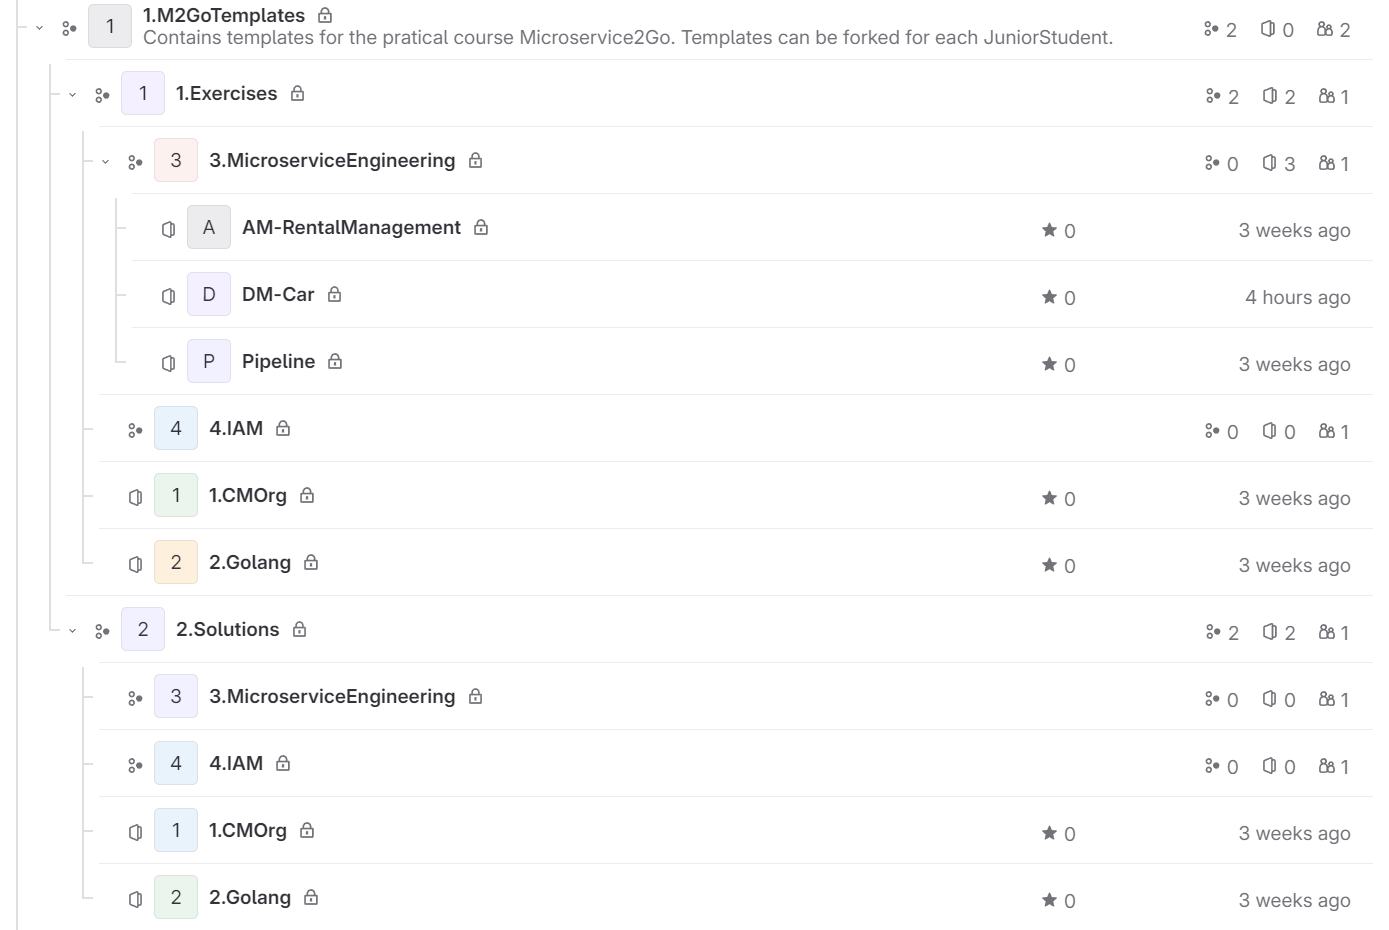
\includegraphics[width=\textwidth]{figures/m2go_templates_gitlab.png}
	\caption{M2Go Templates GitLab Repository Structure \cite{CM-G-M2G}}
	\label{fig:m2go_templates_gitlab}
\end{figure}

\section{Contributions to the Practical Course Microservice2Go}
\label{sec:m2g_contribution}

As a part of this thesis, the author contributed to the M2Go course. The
contributions were focused on the third part of the course: Microservice
Engineering. This part amongst other things focuses on the development of a
domain microservice called DM-Car. Together with a student \cite{La23} who
participated in the WASA2 practical course in 2023, the master solution for
DM-Car was implemented. The master solution is a complete implementation of the
microservice according to the guidelines and best practices of C\&M.
Additionally, exercises were created for the participants of the course based
on this master solution.

\begin{figure}[tb]
	\centering
	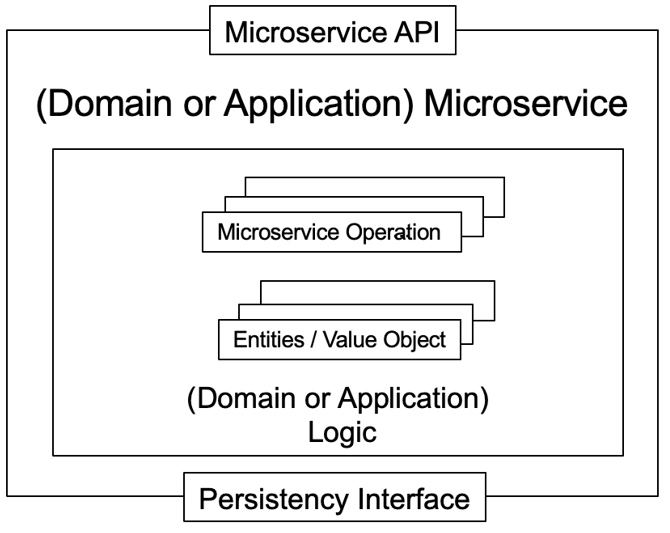
\includegraphics[width=0.5\textwidth]{figures/micro_architecture.png}
	\caption{C\&M Micro Architecture \cite{CM-W-IMP}}
	\label{fig:micro_architecture}
\end{figure}

DM-Car follows the UME approach which was discussed in Section
\ref{sec:ume_approach}. The UME approach provides a software architecture
called micro architecture for implementing microservices. This micro
architecture can be seen in Figure \ref{fig:micro_architecture}. The micro
architecture splits microservices into three parts the API, the logic, and the
infrastructure. The API part of the micro architecture is responsible for
exposing the microservice's API. The main component of the API part is the
controller which accepts incoming requests, routes them to the logic part, and
sends the response back to the requester. The logic part contains the
microservice's domain logic, called microservice operations, as well as the
necessary entities and value objects which are collectively called models. The
infrastructure part provides the microservice with a persistency interface to
allow it to access databases or other forms of storage. The persistence
interface is implemented in the form of a repository that provides basic
functions to access and store data. These are then used by the microservice
operations. The micro architecture also provides the file structure for the
microservice. Each part of the micro architecture gets a separate top-level
directory. The API directory also contains separate directories for the
microservice operations and the models.

\begin{figure}[tb]
	\centering
	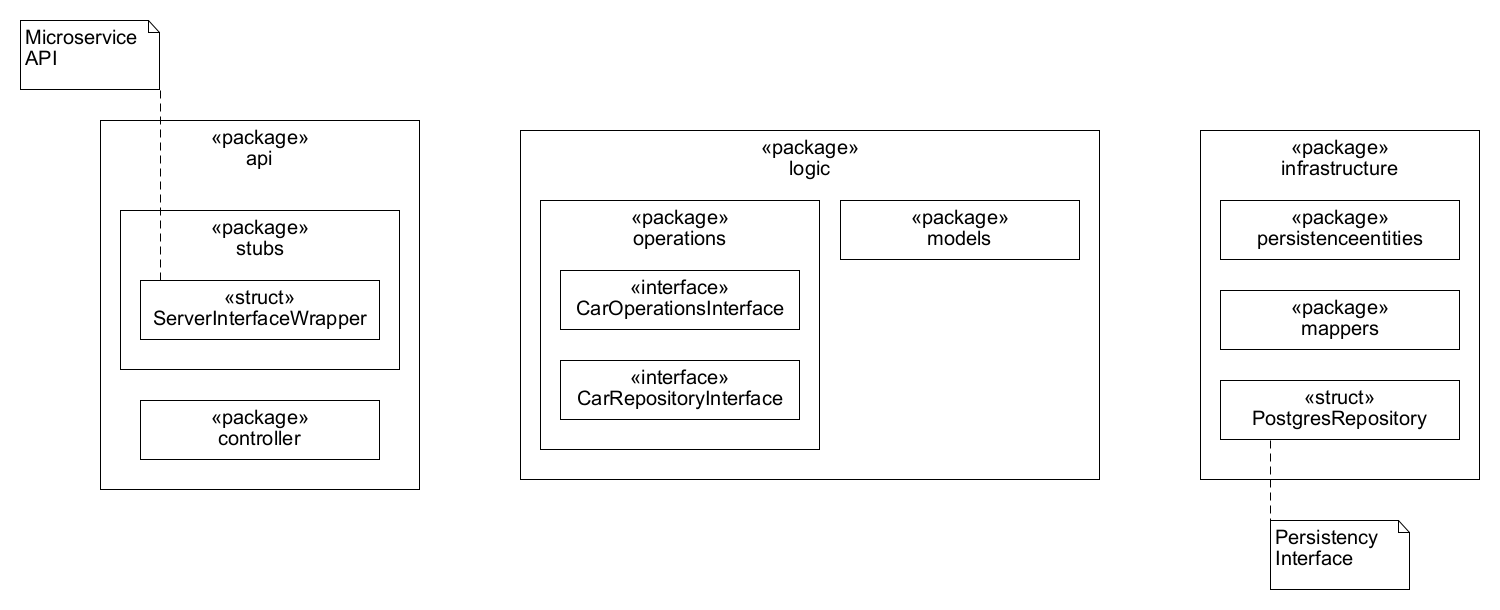
\includegraphics[width=\textwidth]{figures/dm_car_package_structure.png}
	\caption{DM-Car Package Structure}
	\label{fig:dm_car_package_structure}
\end{figure}

DM-Car is split into three packages: api, logic, and infrastructure following
the micro architecture. An overview of DM-Car's package structure can be
seen in Figure \ref{fig:dm_car_package_structure}. The api package contains the
struct ServerInterfaceWrapper that provides DM-Car's API.
The logic package provides the domain logic of DM-Car and includes the sub-packages
operations and models. The models package contains the structs
which model the entities defined in the API diagram. The operations
package contains the CarOperationsInterface which provides the interface
between the API and logic part of DM-Car as well as the CarRepositoryInterface
which provides the interface between the logic and infrastructure part of DM-Car.
The operations package also includes DM-Car's domain logic functions.
The infrastructure package contains the persistency interface of DM-Car through which the
microservice can access persistent storage.

\begin{figure}[tb]
	\centering
	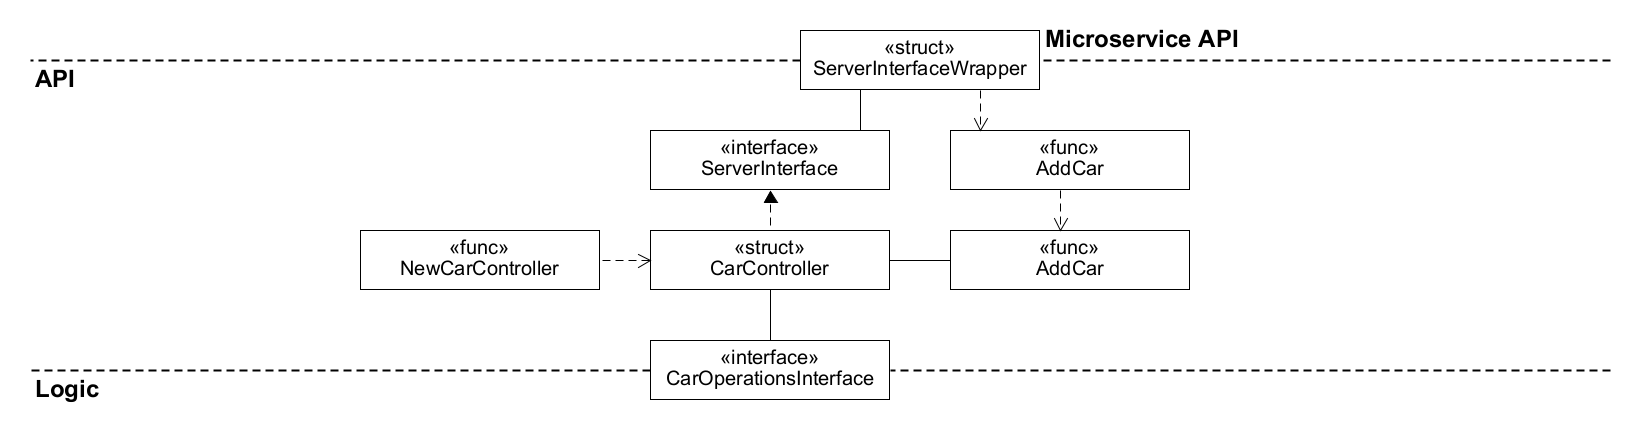
\includegraphics[width=\textwidth]{figures/dm_car_css_api.png}
	\caption{DM-Car Code Structure Sketch: API}
	\label{fig:dm_car_css_api}
\end{figure}

The api package which contains the sub-packages stubs and controller provides the API of DM-Car.
An overview of the api package in the form of a CSS (Code Structure Sketch) can be seen in Listing \ref{fig:dm_car_css_api}.
The stubs package contains code that was generated by the tool oapi-codegen \cite{DEE-OAPI}.
The oapi-codegen tool generates the structure for an HTTP server that uses the Echo framework \cite{LAB-DOCS}
from an API specification written using the OpenAPI standard.
The generated code consists of an interface ServerInterface and a wrapper implementation of that interface
called ServerInterfaceWrapper. The ServiceInterfaceWrapper provides the entry
points for the routes defined in the API specification. Additionally, there is
also a struct Car which implements the model for Car which is defined in the
API specification. The controller package contains the controller CarController
which is the interface between the generated code for the Echo framework and
the implementation of DM-Car. When the server receives a request for one of the
routes defined in the API specification, Echo matches that route to the
corresponding method in the ServerInterfaceWrapper which then calls the method
for that route on the CarController. The methods in CarController handle the
parsing of the incoming data into the corresponding Golang models as well as
parsing the computed response back into JSON which will be returned to the
requester by Echo.

\begin{figure}[tb]
	\centering
	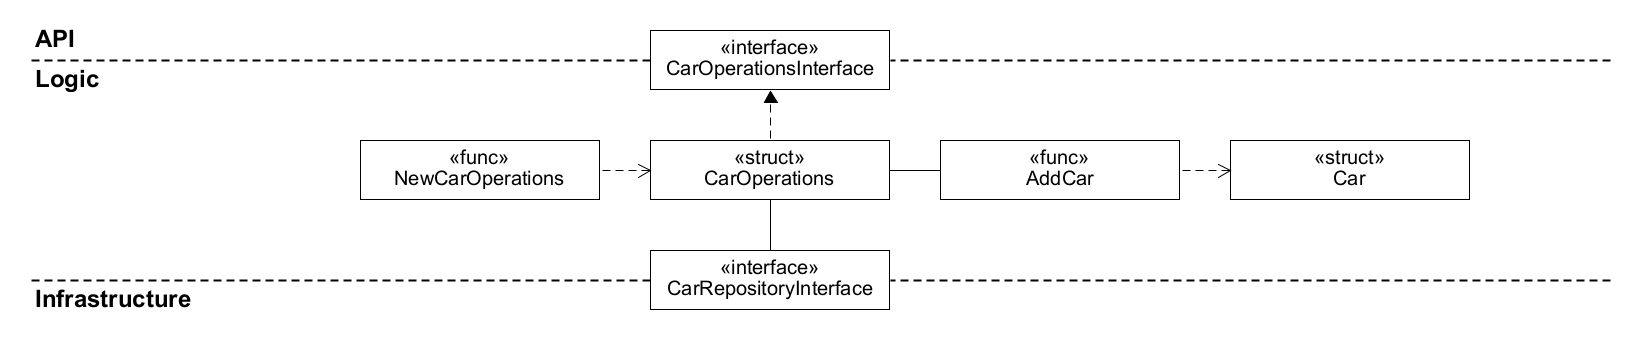
\includegraphics[width=\textwidth]{figures/dm_car_css_logic.png}
	\caption{DM-Car Code Structure Sketch: Logic}
	\label{fig:dm_car_css_logic}
\end{figure}

The logic package which contains the sub-packages operations and models handles
the logic functionality of the server. An overview of the logic package in the form of a CSS (Code Structure Sketch)
can be seen in Listing \ref{fig:dm_car_css_logic}. The models package contains the structs
which model the entities defined in the API diagram. Additionally, the models
package contains the interface CarRepositoryInterface which defines the
interface to the infrastructure part that the logic part of the server expects.
Because the logic part of the server is its central component, it defines both
its interface to be used by the API part as well as the interface to be used by
the infrastructure part. With this approach, the API and infrastructure
components can be exchanged for different implementations without requiring any
changes to the logic part of the server. This is important because the logic
part implements the domain logic which should be agnostic to how the server
receives requests and how data is stored. The API and infrastructure parts
meanwhile have to interact with the server's environment. Therefore they might
need to be adapted, should the environment of the server change, while the
domain logic, defined during the Applications design phase, should be immune
to any such changes. The operations package contains the implementation of the
domain logic.

\begin{figure}[tb]
	\centering
	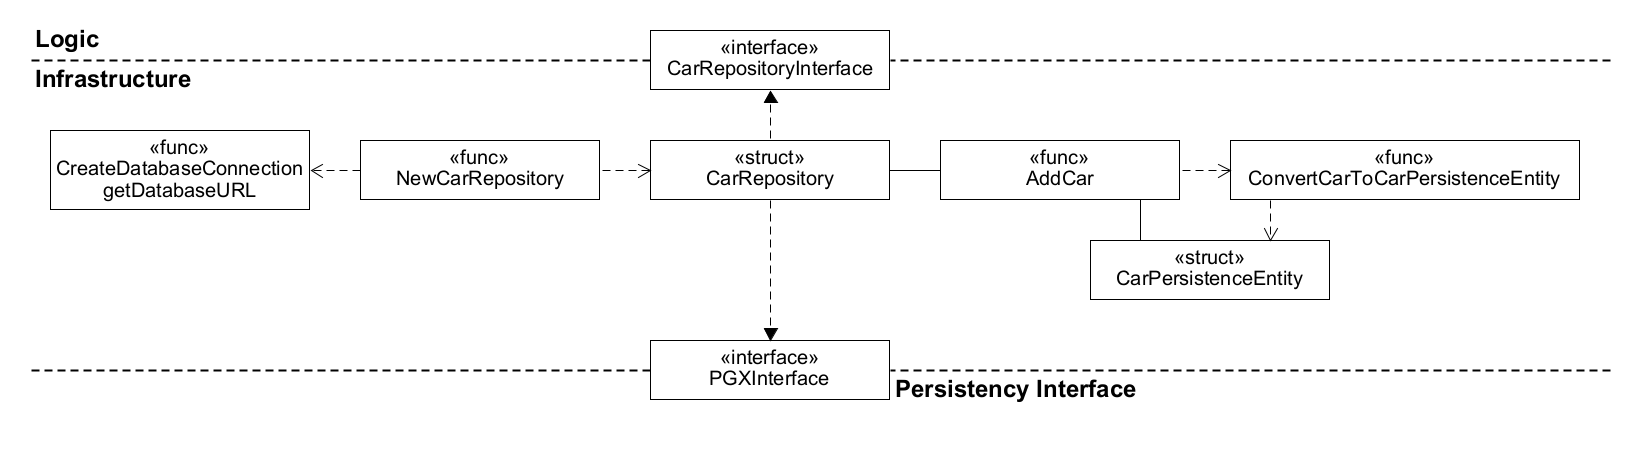
\includegraphics[width=\textwidth]{figures/dm_car_css_infrastructure.png}
	\caption{DM-Car Code Structure Sketch: Infrastructure}
	\label{fig:dm_car_css_infrastructure}
\end{figure}

The infrastructure package contains the sub-packages persistenceentities and mappers.
An overview of the infrastructure package in the form of a CSS (Code Structure Sketch)
can be seen in Listing \ref{fig:dm_car_css_infrastructure}. The
persistenceentities package defines the storage model for the entities of the logic part.
The mappers package contains the struct CarMapper which provides methods to convert
models to persistence entities and vice versa. Additionally, the infrastructure
package contains the struct PostgresRepository which provides the interface between
the server and its storage. In the case of DM-Car, the storage method is a
PostgreSQL \cite{POS-DOCS} database which requires two additional methods to
be present on the PostgresRepository. This is the private method createDatabaseConnection
which establishes a connection to the database and the private method getDatabaseConnectionString which
reads the data necessary to connect to the database from environment variables
and builds a connection string to the database from that data.
To interact with the PostgreSQL database, DM-Car uses the ORM (Object Relational Manager)
GORM \cite{Ji23}.

The logical flow of an incoming request to the server is the following: First, the requests
will be received by Echo through the EchoRouter which decides which method on
the ServerInterfaceWrapper should be called. The ServerInterfaceWrapper then
forwards the request to the correct method on the controller CarController.
CarController parses the request data and forwards the parsed data to
CarOperations. CarOperations performs the requested domain logic on the
provided data, as well as checking that the incoming data conforms to the
domain constraints. While processing the request, CarOperations may utilize
none or several methods on the repository PostgresRepository. The repository
PostgresRepository may load data from the database or write new data to it. After
the request has been processed by CarOperations, the result is returned to
CarController which translates the result into an HTTP response which may
optionally contain a JSON payload. CarController returns this response to the
ServerInterfaceWrapper, which gives the response to Echo so that it can be sent
to the requester.

The initial implementation of DM-Car used an in-memory database which was
directly implemented in the repository InMemoryRepository in the form of a map data structure. The
first task of the author was to replace InMemoryRepository's implementation with an
implementation that utilizes a PostgreSQL database for data storage.
The new for this new repository is PostgresRepository. To connect
to a PostgreSQL database, the GORM library was used. GORM is an ORM which means that it
handles the translation from database tables to Golang structs. GORM also provides
functionality to automatically create database tables that represent the structs that should
be stored in the database. This functionality is called auto migrations.
The implementation of how DM-Car establishes a connection to a database can be seen
in the CSS in Listing \ref{fig:create_db_connection_css}. To connect to a
PostgreSQL database, the repository PostgresRepository calls the method
createDatabaseConnection during its creation.
createDatabaseConnection returns an object through which actions on the database can be performed or an error if
the connection cannot be established. First, createDatabaseConnection calls the
method getDatabaseConnectionString which computes the connection string through which GORM
can reach the database. To compute the correct connection string, getDatabaseConnectionString reads the following
environment variables: POSTGRES\_USER, POSTGRES\_PASSWORD,
POSTGRES\_HOST, POSTGRES\_PORT, and POSTGRES\_DATABASE. These values are used to construct the connection string that has the following format:
\"host=POSTGRES\_HOST user=POSTGRES\_USER password=POSTGRES\_PASSWORD dbname=POSTGRES\_DATABASE port=POSTGRES\_PORT\",
where POSTGRES\_USER and POSTGRES\_PASSWORD are the credentials of an account registered with the database.
POSTGRES\_HOST and POSTGRES\_PORT are the URL where the database can be reached and POSTGRES\_DATABASE is the name of the database.
After getting the connection string for the database, createDatabaseConnection calls the method
gorm.Open with the previously computed connection string.
This returns an object through which DM-Car can interact with the database via GORM.
This object is then stored in the PostgresRepository struct.
In the case that the connection fails, the method is exited early and an error is returned to the
caller of createDatabaseConnection.

\begin{figure}[tb]
	\centering
	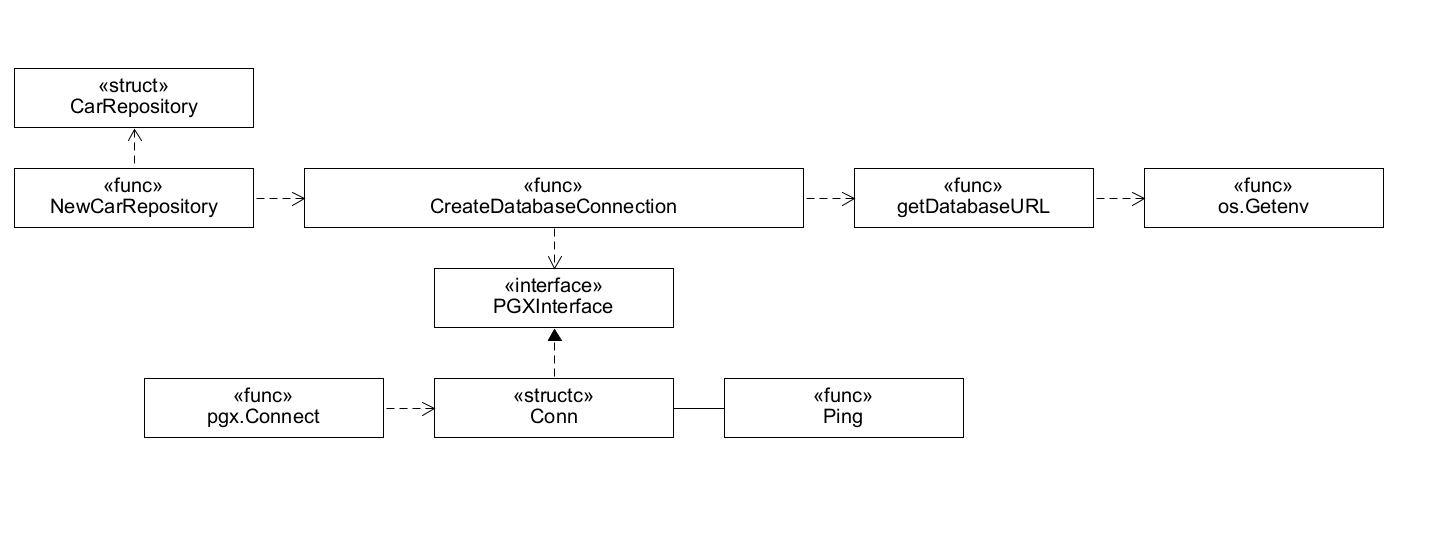
\includegraphics[width=\textwidth]{figures/CreateDatabaseConnectionCSS.png}
	\caption{DM-Car Code Structure Sketch: createDatabaseConnection}
	\label{fig:create_db_connection_css}
\end{figure}

An overview of PostgresRepository's methods AddCar, GetCar, and GetCars in the form of CSS diagrams
can be seen in Listings \ref{fig:add_car_css}, \ref{fig:get_car_css}, and \ref{fig:get_cars_css}.

Listing \ref{fig:add_car_css} shows the CSS diagram of PostgresRepository's AddCar method.
The function AddCar receives a car model from the logic part of DM-Car as an input.
This car model is first converted to a car persistence entity using the ConvertCarToCarPersistenceEntity
method from the mappers package.
This car persistence entity is then passed to the method Create of GORM which persists data that it's being passed
into the connected database.

\begin{figure}[tb]
	\centering
	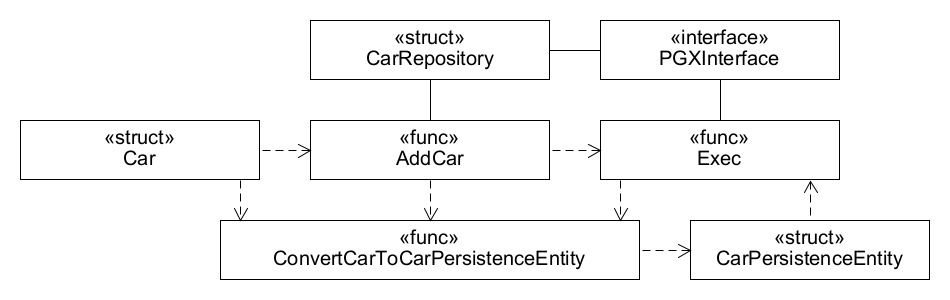
\includegraphics[width=\textwidth]{figures/AddCarCSS.png}
	\caption{DM-Car Code Structure Sketch: AddCar}
	\label{fig:add_car_css}
\end{figure}

Listing \ref{fig:get_car_css} shows the CSS diagram of PostgresRepository's GetCar method.
GetCar retrieves a car by its VIN from the database.
The function GetCar receives a VIN model from the logic part of DM-Car as an input.
GORM provides a method called First for reading one row of data from a database.
The method First receives an empty struct as an input. GORM then returns the first row
of data from the table in the database that is associated with the struct's type.
The returned data is placed into the empty struct. To use more complex queries in GORM,
different methods can be chained together. The method Where from GORM can be chained
with the method First to add a SQL WHERE clause to the query.
This is used by GetCar to filter for cars whose VIN matches the VIN that it received as an input.
Because the domain constraints state that a VIN should be unique, this is expected to return at most
one result which is why the method First is used to read the data that GORM found.
The result is put into an empty CarPersistenceEntity struct by GORM which is passed to the First method as an argument.
After the query to the database completes, GORM puts the resulting data into the provided struct.
This car persistence entity is then converted to a car model for the logic part of DM-Car
using the method ConvertCarPersistenceEntityToCar from the mappers package.
Finally, the car model is returned as a result from the GetCar method.

\begin{figure}[tb]
	\centering
	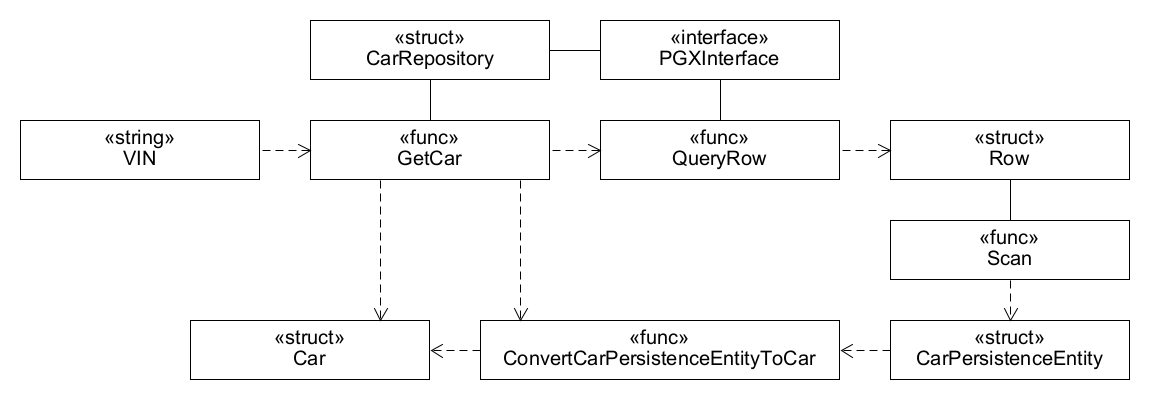
\includegraphics[width=\textwidth]{figures/GetCarCSS.png}
	\caption{DM-Car Code Structure Sketch: GetCar}
	\label{fig:get_car_css}
\end{figure}

Listing \ref{fig:get_cars_css} shows the CSS diagram of PostgresRepository's GetCars method.
GetCars retrieves all cars stored in the database.
Another method that GORM provides for reading data from the connected database is the Find method.
The Find method works similarly to the First method but instead of returning at most one row of data,
the Find method can return multiple rows of data. Because GetCars should retrieve all cars
from the database, there is no need to chain a call to the Where method to the call to the Find method.
The Find method receives an array of empty structs into which GORM places the query results.
This array is then converted to a Cars model which contains multiple Car models.
The conversion is performed by the function ConvertCarPersistenceEntitiesToCars from the mappers package.

\begin{figure}[tb]
	\centering
	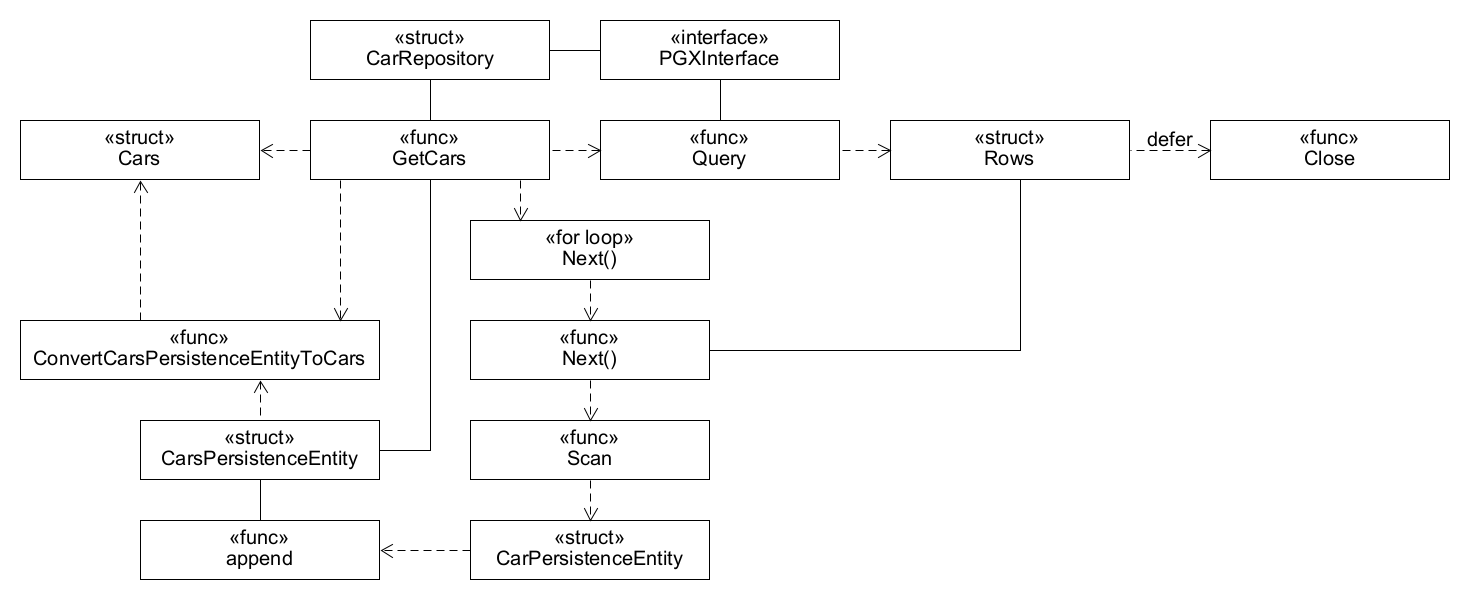
\includegraphics[width=\textwidth]{figures/GetCarsCSS.png}
	\caption{DM-Car Code Structure Sketch: GetCars}
	\label{fig:get_cars_css}
\end{figure}

\section{Description of the DM-Car Exercises}
\label{sec:m2g_description_exercises}

% TODO: aufgaben beschreibungen: was sollen die

\section{Implementation of DM-Car}
\label{sec:m2g_exercise}

The UME approach uses C\&M's micro architecture to implement microservices.
This micro architecture is described in the chapter Implementation and Test of
the WASA course unit Microservice Engineering \cite{CM-W-IMP}. The DM-Car implementation, which
is to be investigated, can be found in the C\&M GitLab in 1\_1.M2Go >
1.M2GoTemplates > 1.Exercises > 3.MicroserviceEngineering > DM-Car \cite{CM-G-DMC}.

\fbox{\parbox{\textwidth}{
\textbf{Exercise MicroArchDMCar}
\begin{enumerate}
	\item \textbf{The UME Micro Architecture} \\
	What are the three parts of a micro architecture
	and which aspect does each part cover in a microservice implementation?

	\item \textbf{Usage of the Micro Architecture} \\
	To which parts of the micro architecture do the following structs and interfaces
	in DM-Car belong: CarController \cite{CM-G-CON}, CarOperationsInterface \cite{CM-G-IOP}, CarOperations \cite{CM-G-OP},
	GetCarOperation \cite{CM-G-GET}, CarRepositoryInterface \cite{CM-G-IREPO}, and InMemoryRepository \cite{CM-G-MEMREPO}.
	Add a figure to your practical course thesis which graphically illustrates the relation
	between these components of DM-Car and the micro architecture.
\end{enumerate}
}}

The chapter Implementation and Test of the WASA course unit Microservice Engineering \cite{CM-W-IMP}
introduces the concept of a CSS (Code Structure Sketch) which can be used
to visualize the structure of the source code and bridge the gap between the design
artifacts like class diagrams and the actual implementation.

\fbox{\parbox{\textwidth}{
\textbf{Exercise ImplementationDMCar}
\begin{enumerate}
	\item \textbf{Code Structure Sketches} \\
	Create Code Structure Sketches in your practical course thesis
	that visualize the implementation of the method GetCar in the CarController \cite{CM-G-CON},
	the GetCarOperation \cite{CM-G-GET}, and the method GetCar in the InMemoryRepository \cite{CM-G-MEMREPO}.
	
	\item \textbf{Control Flow of DM-Car} \\
	Describe the code structure of DM-Car by explaining the flow
	of the method GetCar in the CarController \cite{CM-G-CON} from its invocation
	until its return. Use the previously created Code Structure Sketches
	for your description.
\end{enumerate}
}}

The tool Postman can be used to send requests to microservices. An overview of the tool
can be found in the UME Best Practice: Implementing a Microservice in Golang \cite{CM-G-BEIMPL}.

\fbox{\parbox{\textwidth}{
\textbf{Challenge ExtendingDMCar}
\begin{enumerate}
	\item \textbf{Extending the API Specification} \\
	Extend the API specification of DM-Car \cite{CM-G-API} with the method addCar()
	described in the API diagram of DM-Car.

	\item \textbf{Generate Server Stubs From API Specification} \\
	Regenerate the stubs in DM-Car from the new API specification
	using the oapi-codegen tool \cite{DEE-OAPI}.

	\item \textbf{Documentation} \\
	Document the changes to the source code of DM-Car caused by the previous task
	in your practical course thesis.

	\item \textbf{API Controller Implementation} \\
	Implement the method AddCar in the API Controller CarController \cite{CM-G-CON}.

	\item \textbf{Microservice Operation Implementation} \\
	Implement the AddCarOperation.

	\item \textbf{Repository Implementation} \\
	Implement the method AddCar in the repository InMemoryRepository \cite{CM-G-MEMREPO}.

	\item \textbf{Testing the Implementation} \\
	Test your implementation of the new InMemoryRepository by creating three cars
	with requests sent via Postman \cite{CM-G-BEIMPL}. Document the requests that you used and their responses in your practical
	course thesis.
\end{enumerate}
}}

\section{Infrastructure Implementation of DM-Car}
\label{sec:m2g_infrastructure}

The Golang library GORM \cite{Ji23} provides an ORM (Object Relational Manager)
to interact with PostgreSQL databases from a Golang application. An overview of the library can be found
in the UME Best Practice: Implementing a Microservice in Golang \cite{CM-G-BEIMPL}.

\fbox{\parbox{\textwidth}{
\textbf{Challenge InfrastructureDMCar}
\begin{enumerate}
	\item \textbf{Setting up a New Repository} \\
	Create a new repository for DM-Car called PostgresRepository in the infrastructure package \cite{CM-G-INFRA}.
	Add method stubs to PostgresRepository that implement the interface CarRepositoryInterface \cite{CM-G-IREPO}.

	\item \textbf{Reading Environment Variables} \\
	Add a function to the PostgresRepository that reads the values of the environment variables
	POSTGRES\_HOST, POSTGRES\_PORT, POSTGRES\_USER, POSTGRES\_PASSWORD, and POSTGRES\_NAME. Combine the values of these
	environment values into a string with the following format that is returned by your function:
	\"host=POSTGRES\_HOST user=POSTGRES\_USER password=POSTGRES\_PASSWORD dbname=POSTGRES\_DATABASE port=POSTGRES\_PORT\",

	\item \textbf{Connecting to a Database} \\
	Create a method NewPostgresRepository that constructs a new PostgresRepository and
	connects DM-Car to a PostgreSQL database. To communicate with a PostgreSQL database,
	the GORM library should be used \cite{CM-G-BEIMPL}.
	Store the returned connection object in the PostgresRepository struct.

	\item \textbf{Database Repository: AddCar} \\
	Implement the method AddCar in PostgresRepository that uses the database
	to create and store cars.

	\item \textbf{Database Repository: GetCar} \\
	Implement the method GetCar in PostgresRepository that uses the database
	to get a car by its VIN.

	\item \textbf{Database Repository: GetCars} \\
	Implement the method GetCars in PostgresRepository that uses the database
	to retrieve all stored cars.

	\item \textbf{Using the New Repository} \\
	Create an instance of PostgresRepository in DM-Car's main method \cite{CM-G-MAIN}
	and use that instance instead of the InMemoryDatabase to create a new instance of CarOperations.

	\item \textbf{Documentation} \\
	Test your implementation of PostgresRepository by creating three cars with requests sent to DM-Car
	via Postman \cite{CM-G-BEIMPL}.
	Next, create a request to retrieve one of those cars by its VIN and one request to retrieve
	all existing cars. Document the requests that you used and their responses in your practical
	course thesis.
\end{enumerate}
}}

\section{Solutions to the DM-Car Exercises}
\label{sec:m2g_solutions}

This section contains the solutions to the exercises in Section \ref{sec:m2g_exercise}
and Section \ref{sec:m2g_infrastructure}. The solutions are in the same order as the exercises.

\subsection*{Exercise MicroArchDMCar - Solutions}

The solution to the exercise The UME Micro Architecture can be found in the WASA lecture in the
chapter Microservice Engineering 5 - Implementation and Test \cite{CM-W-IMP}.

The solution to the exercise Usage of the Micro Architecture can be seen in Figure \ref{fig:m2go_solution_1_2}.
CarController belongs to the Microservice API of the micro architecture as it provides the microservice's API.
CarOperationsInterface provides the interface between the API and logic parts of the microservice.
CarOperations and GetCarOperation are both part of the logic part of the microservice.
CarRepositoryInterface provides the persistency interface to interact with InMemoryRepository
which in this case represents the database being used by the microservice.

\begin{figure}[tb]
	\centering
	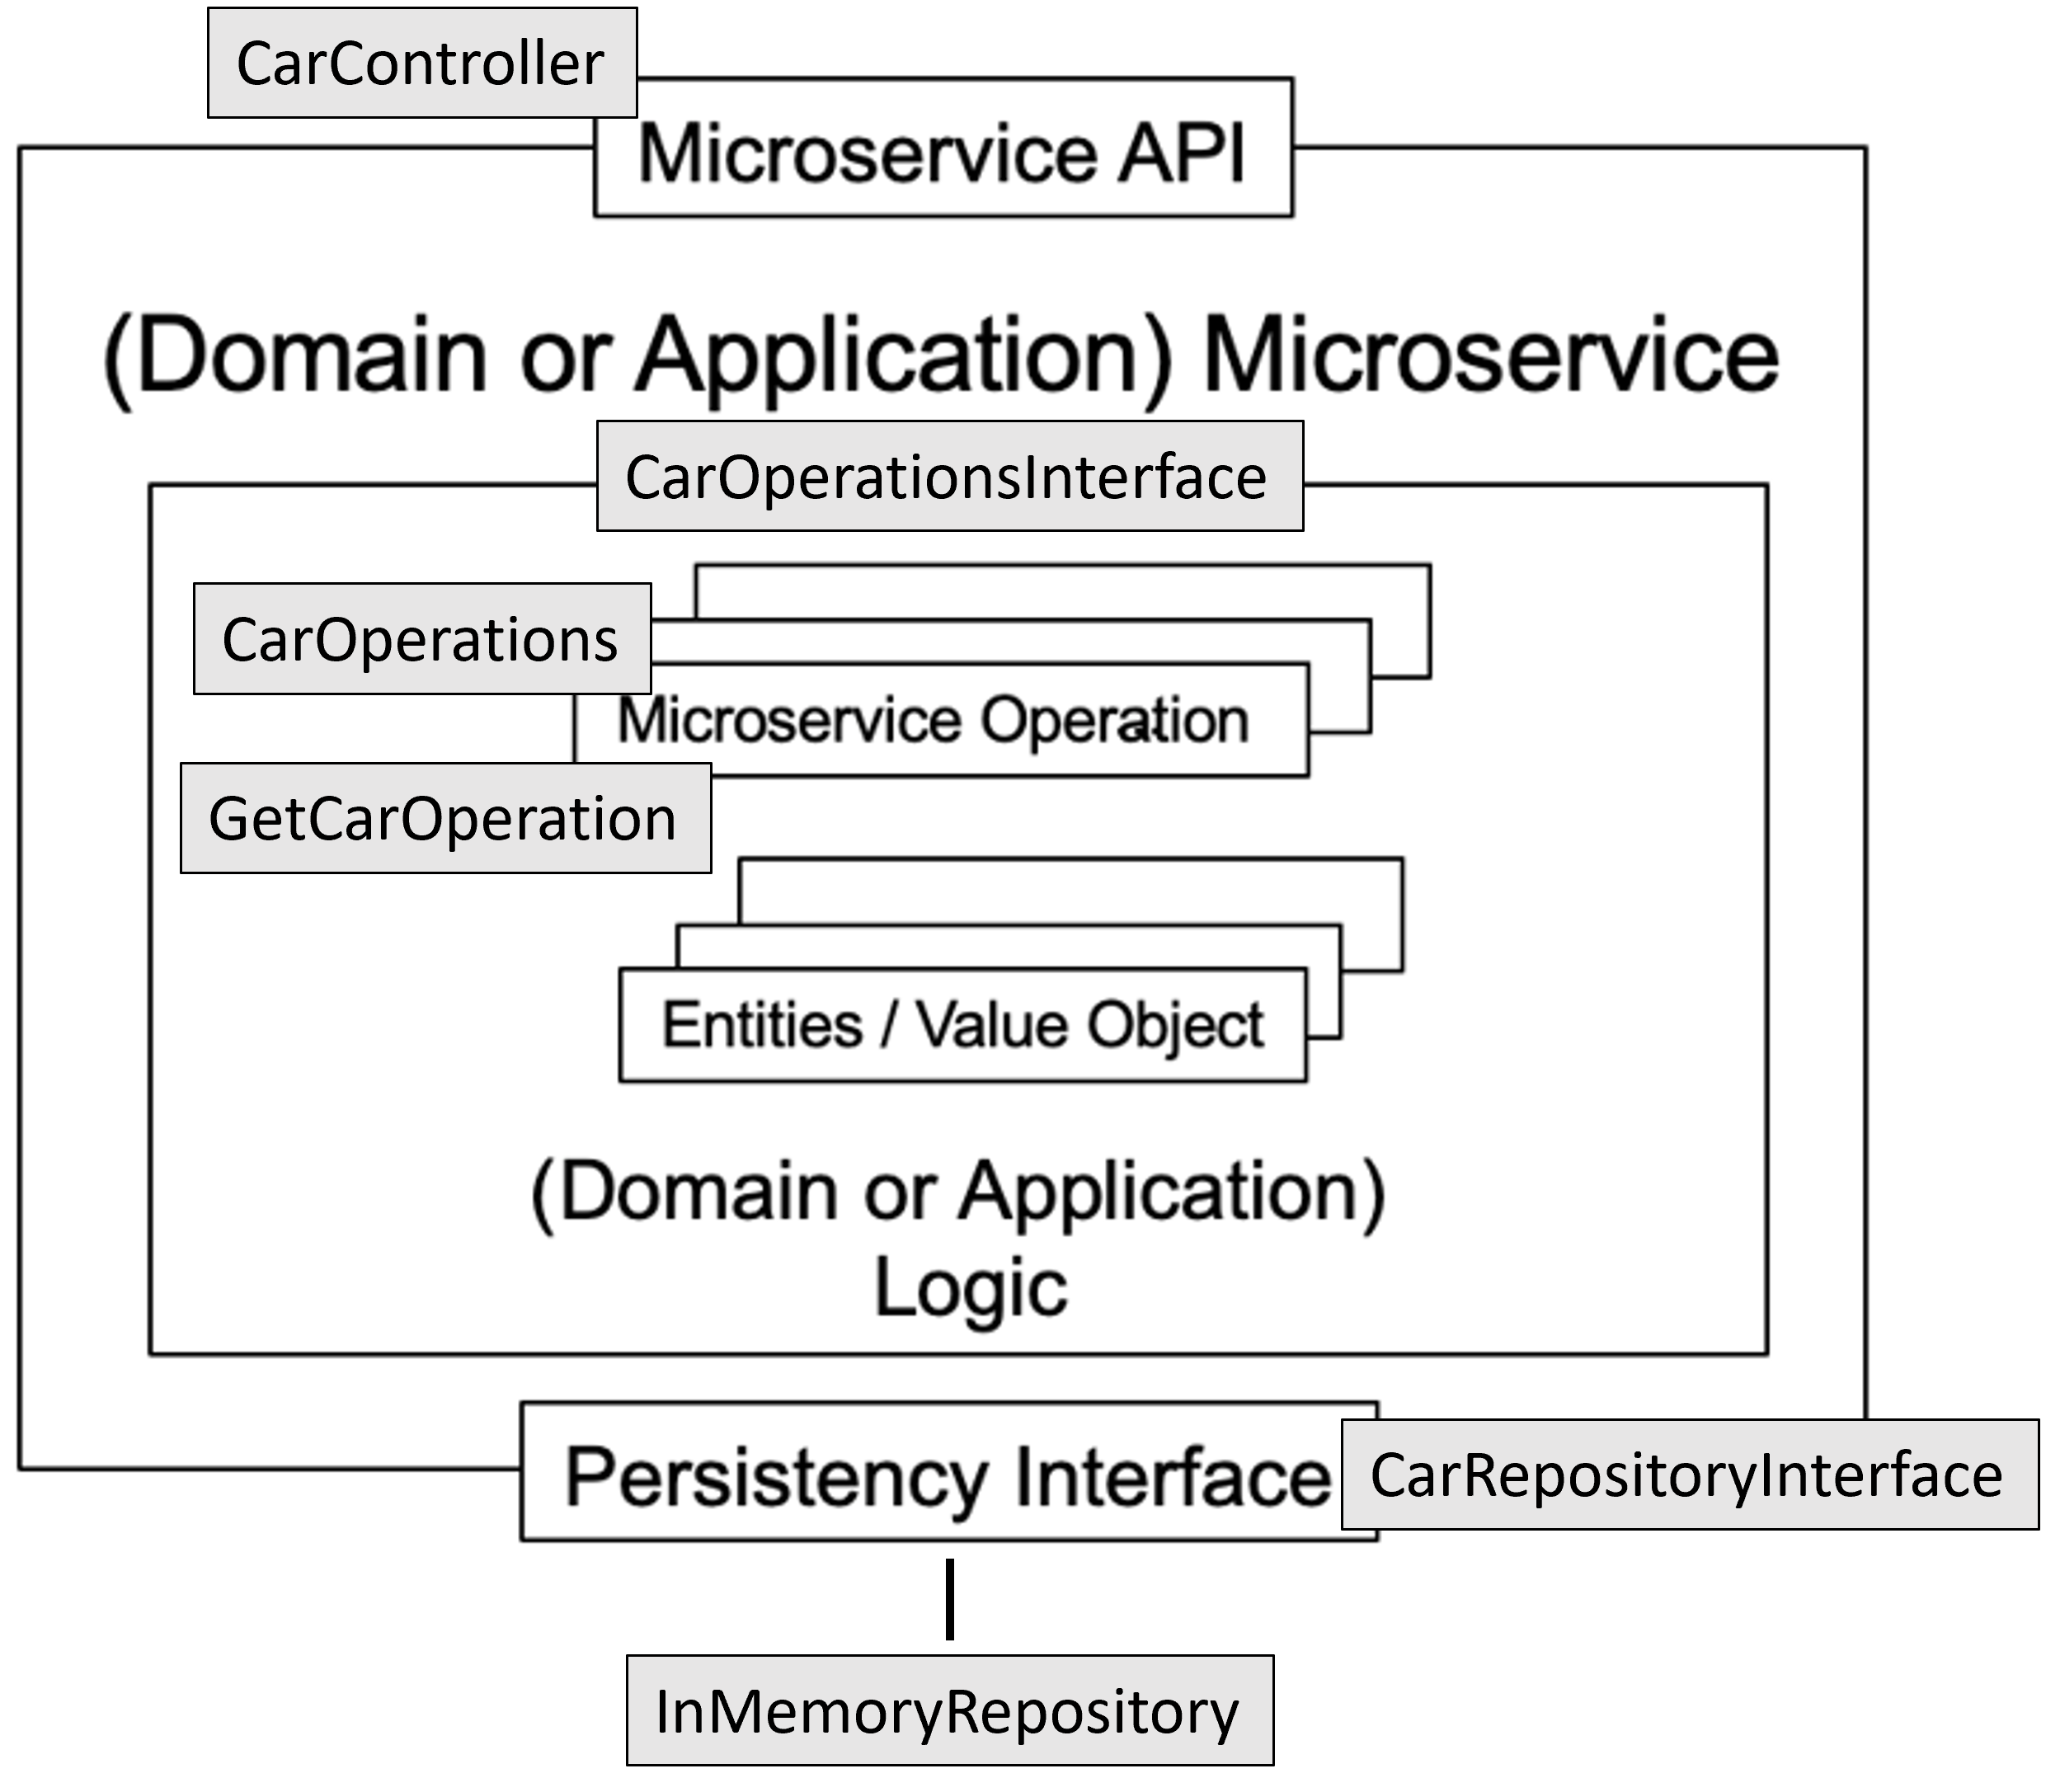
\includegraphics[width=0.7\textwidth]{figures/m2go_solution_1_2.png}
	\caption{Exercise MicroArchDMCar - Usage of the Micro Architecture Solution}
	\label{fig:m2go_solution_1_2}
\end{figure}

\subsection*{Exercise ImplementationDMCar - Solutions}

Figure \ref{fig:m2go_carcontroller_getcar_css} shows the solution for the CSS of the CarController's GetCar method.

\begin{figure}[tb]
	\centering
	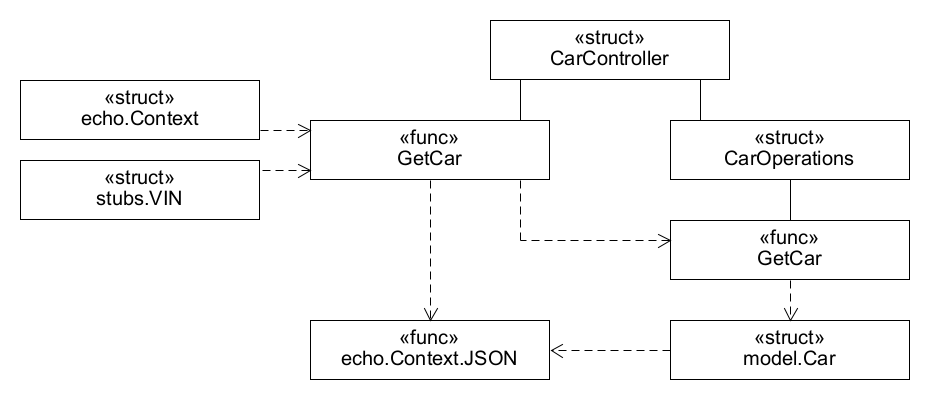
\includegraphics[width=0.7\textwidth]{figures/m2go_carcontroller_getcar_css.png}
	\caption{Exercise ImplementationDMCar - CarController GetCar CSS Solution}
	\label{fig:m2go_carcontroller_getcar_css}
\end{figure}

Figure \ref{fig:m2go_caroperations_getcar_css} shows the solution for the CSS of the CarOperation's GetCarOperation method.

\begin{figure}[tb]
	\centering
	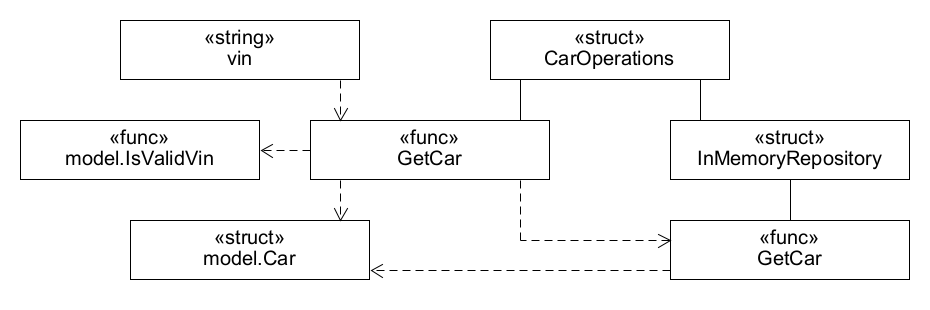
\includegraphics[width=0.7\textwidth]{figures/m2go_caroperations_getcar_css.png}
	\caption{Exercise ImplementationDMCar - GetCarOperation CSS Solution}
	\label{fig:m2go_caroperations_getcar_css}
\end{figure}

Figure \ref{fig:m2go_inmemoryrepository_getcar_css} shows the solution for the CSS of the InMemoryRepository's GetCar method.

\begin{figure}[tb]
	\centering
	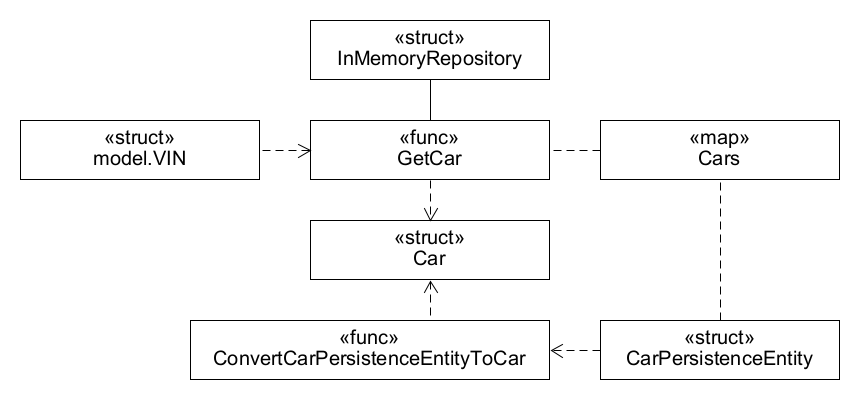
\includegraphics[width=0.7\textwidth]{figures/m2go_inmemoryrepository_getcar_css.png}
	\caption{Exercise ImplementationDMCar - InMemoryRepository GetCar CSS Solution}
	\label{fig:m2go_inmemoryrepository_getcar_css}
\end{figure}

The following is the solution to the task Control Flow of DM-Car from the ImplementationDMCar exercise:
The logical flow of an incoming request to the server is the following: First, the requests
will be received by Echo through the EchoRouter which decides which method on
the CarController should be called with the data parsed from the request.
CarController forwards the request to the correct car operation.
In the case of the CarController's GetCar method, which is invoked with the current
context of the Echo framework and the VIN that was contained in the request,
the GetCarOperation is called with the received VIN. CarOperations performs the requested domain logic
on the provided data, as well as checking that the incoming data conforms to the
domain constraints. While processing the request, CarOperations may utilize
none or several methods on the repository InMemoryRepository.
In the case of the GetCarOperation, the VIN is tested to see if it conforms
to the domain constraints. If the VIN is valid, GetCarOperation calls the GetCar method
on the InMemoryRepository with the VIN as an argument.
The InMemoryRepository's GetCar method tries to retrieve a car by the provided VIN from its internal map
and return it.
If no car with a matching VIN could be found, the method returns an error and an empty Car struct.
The result from the InMemoryRepository's GetCar method is then returned to the GetCarOperation.
If GetCarOperation receives an error from InMemoryRepository then it propagates the error
to CarController. Otherwise, it returns the car that was found to CarController.
Lastly, CarController also checks if it received an error from the GetCarOperation.
In that case, CarController returns an error to the Echo framework which is forwarded to the sender of the original request.
Otherwise, CarController sets the found car as the body of the HTTP response in JSON format along
with the status code HTTP 200 (OK). This response is then sent to the requester by Echo.

\subsection*{Challenge ExtendingDMCar - Solutions}

The solutions to tasks 1 to 7 can be found in the master solution for DM-Car \cite{CM-G-DMC}.

The solution to the task Testing the Implementation can be seen in Listing \ref{lis:m2go_solution_3_7}.
The \$PORT in the Listing should be the port that the microservice was running on
when sending the requests.
The three requests in the Listing create cars using the HTTP POST method on the route /cars.
The data for these cars is taken from the Section API Design of DM-Car in the exercise document.

\begin{lstlisting}[caption = {Challenge ExtendingDMCar - Testing the Implementation}, label = {lis:m2go_solution_3_7}, style = kit-cm, language=]
Request: POST localhost:$PORT/cars
{
   "vin": "JH4DB1561NS000565",
   "brand": "Honda",
   "model": "Acura"
}
Response: HTTP 200 - OK
{
  "Vin": {
    "Vin": "JH4DB1561NS000565"
  },
  "Brand": "Honda",
  "Model": "Acura"
}
--------
Request: POST localhost:$PORT/cars
{
   "vin": "JN8AZ2NC5B9300256",
   "brand": "Nissan",
   "model": "Infiniti"
}
Response: HTTP 200 - OK
{
  "Vin": {
    "Vin": "JN8AZ2NC5B9300256"
  },
  "Brand": "Nissan",
  "Model": "Infiniti"
}
--------
Request: POST localhost:$PORT/cars
{
   "vin": "2FDKF38G3KCA42390",
   "brand": "Ford",
   "model": "F350"
}
Response: HTTP 200 - OK
{
  "Vin": {
    "Vin": "2FDKF38G3KCA42390"
  },
  "Brand": "Ford",
  "Model": "F350"
}
\end{lstlisting}

\subsection*{Challenge InfrastructureDMCar - Solutions}

The solutions to tasks 1 to 7 can be found in the master solution for DM-Car \cite{CM-G-DMC}.

The partial solution to the task Documentation can be seen in Listing \ref{lis:m2go_solution_4_8}.
The \$PORT in the Listing should be the port that the microservice was running on
when sending the requests.
The solution for the requests to create cars can be found in Listing \ref{lis:m2go_solution_3_7}
from the solutions to Challenge ExtendingDMCar.
The first request in the Listing uses the HTTP GET method on the route /cars/:VIN to retrieve the car that was created using the first request.
The second request in the Listing retrieves all cars using the HTTP GET method at the route /cars.

\begin{lstlisting}[caption = {Challenge InfrastructureDMCar - Documentation}, label = {lis:m2go_solution_4_8}, style = kit-cm, language=]
Request: GET localhost:$PORT/cars/JH4DB1561NS000565
Response: HTTP 200 - OK
{
  "Vin": {
    "Vin": "JH4DB1561NS000565"
  },
  "Brand": "Honda",
  "Model": "Acura"
}
--------
Request: GET localhost:$PORT/cars
Response: HTTP 200 - OK
{
  "Cars": [
    {
      "Vin": {
        "Vin": "JH4DB1561NS000565"
      },
      "Brand": "Honda",
      "Model": "Acura"
    },
    {
      "Vin": {
        "Vin": "JN8AZ2NC5B9300256"
      },
      "Brand": "Nissan",
      "Model": "Infiniti"
    },
    {
      "Vin": {
        "Vin": "2FDKF38G3KCA42390"
      },
      "Brand": "Ford",
      "Model": "F350"
    }
  ]
}
\end{lstlisting}